

CatCode was originally developed using a text editor; however, due to the modular structure of the CatCode systems, this could be swapped out for the graphical editor. The graphical editor handles editing and compilation, is shown in \autoref{fig:design/catCode-example-graphical}, and is available in: \texttt{res://src/catCode/ui/basic\_graphical\_editor}.

\begin{figure}
    \centering
    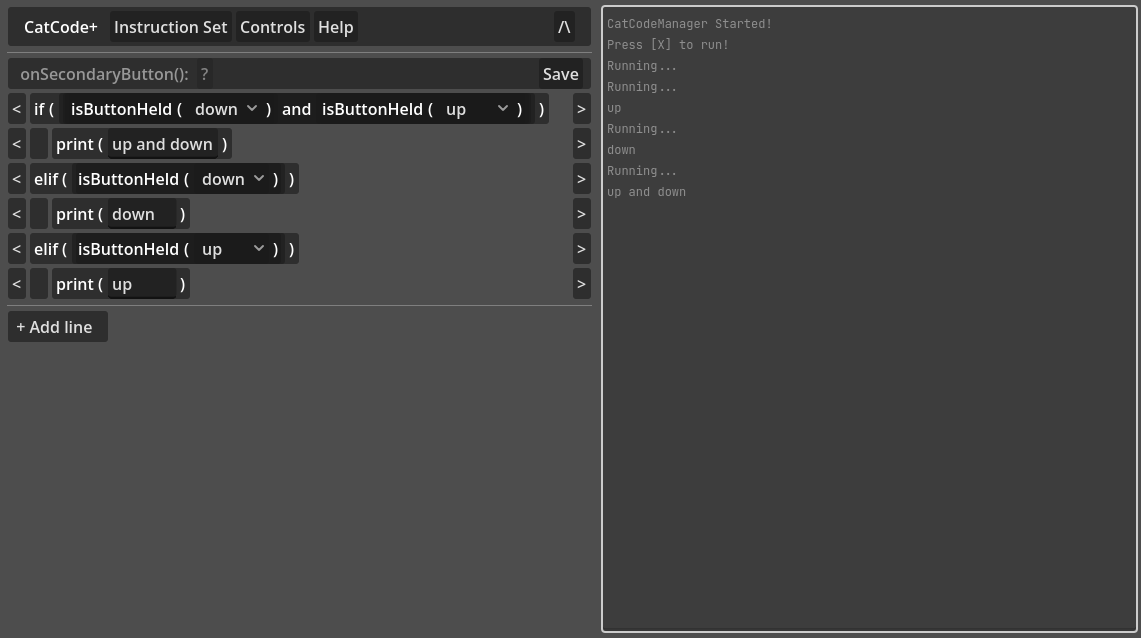
\includegraphics[width=0.75\linewidth]{C5//GraphicalCatCode/basicGraphicalIDEexample.png}
    \caption[Example graphical catCode]{Example graphical catCode, taken from \texttt{res://levels/test/gui\_basic\_ide.tscn}}
    \label{fig:design/catCode-example-graphical}
\end{figure}

\subsection{Structure}

The graphical editor relies \textit{HBox} and \textit{VBox} nodes, which automatically align nodes in the order they are instanced in the node tree. The structure of these nodes are shown in \autoref{fig:design/catCode-graphicalEditor-Nodes} This was choice, alongside all the others for designing this UI were pragmatic and made under the assumption that aesthetics (such are colour and font) and form would be improved later in development.

There are three main components:
\begin{enumerate}
    \item The \textbf{header bar} which contains buttons that show documentation and help menus.
    \item The \textbf{function header} which says when the script is executed.
    \item The \textbf{code container} which contains \textit{GraphicalBlock} instances as children and is where script editing is undertaken. 
\end{enumerate}

\begin{fullwidthfigure}
    \centering
    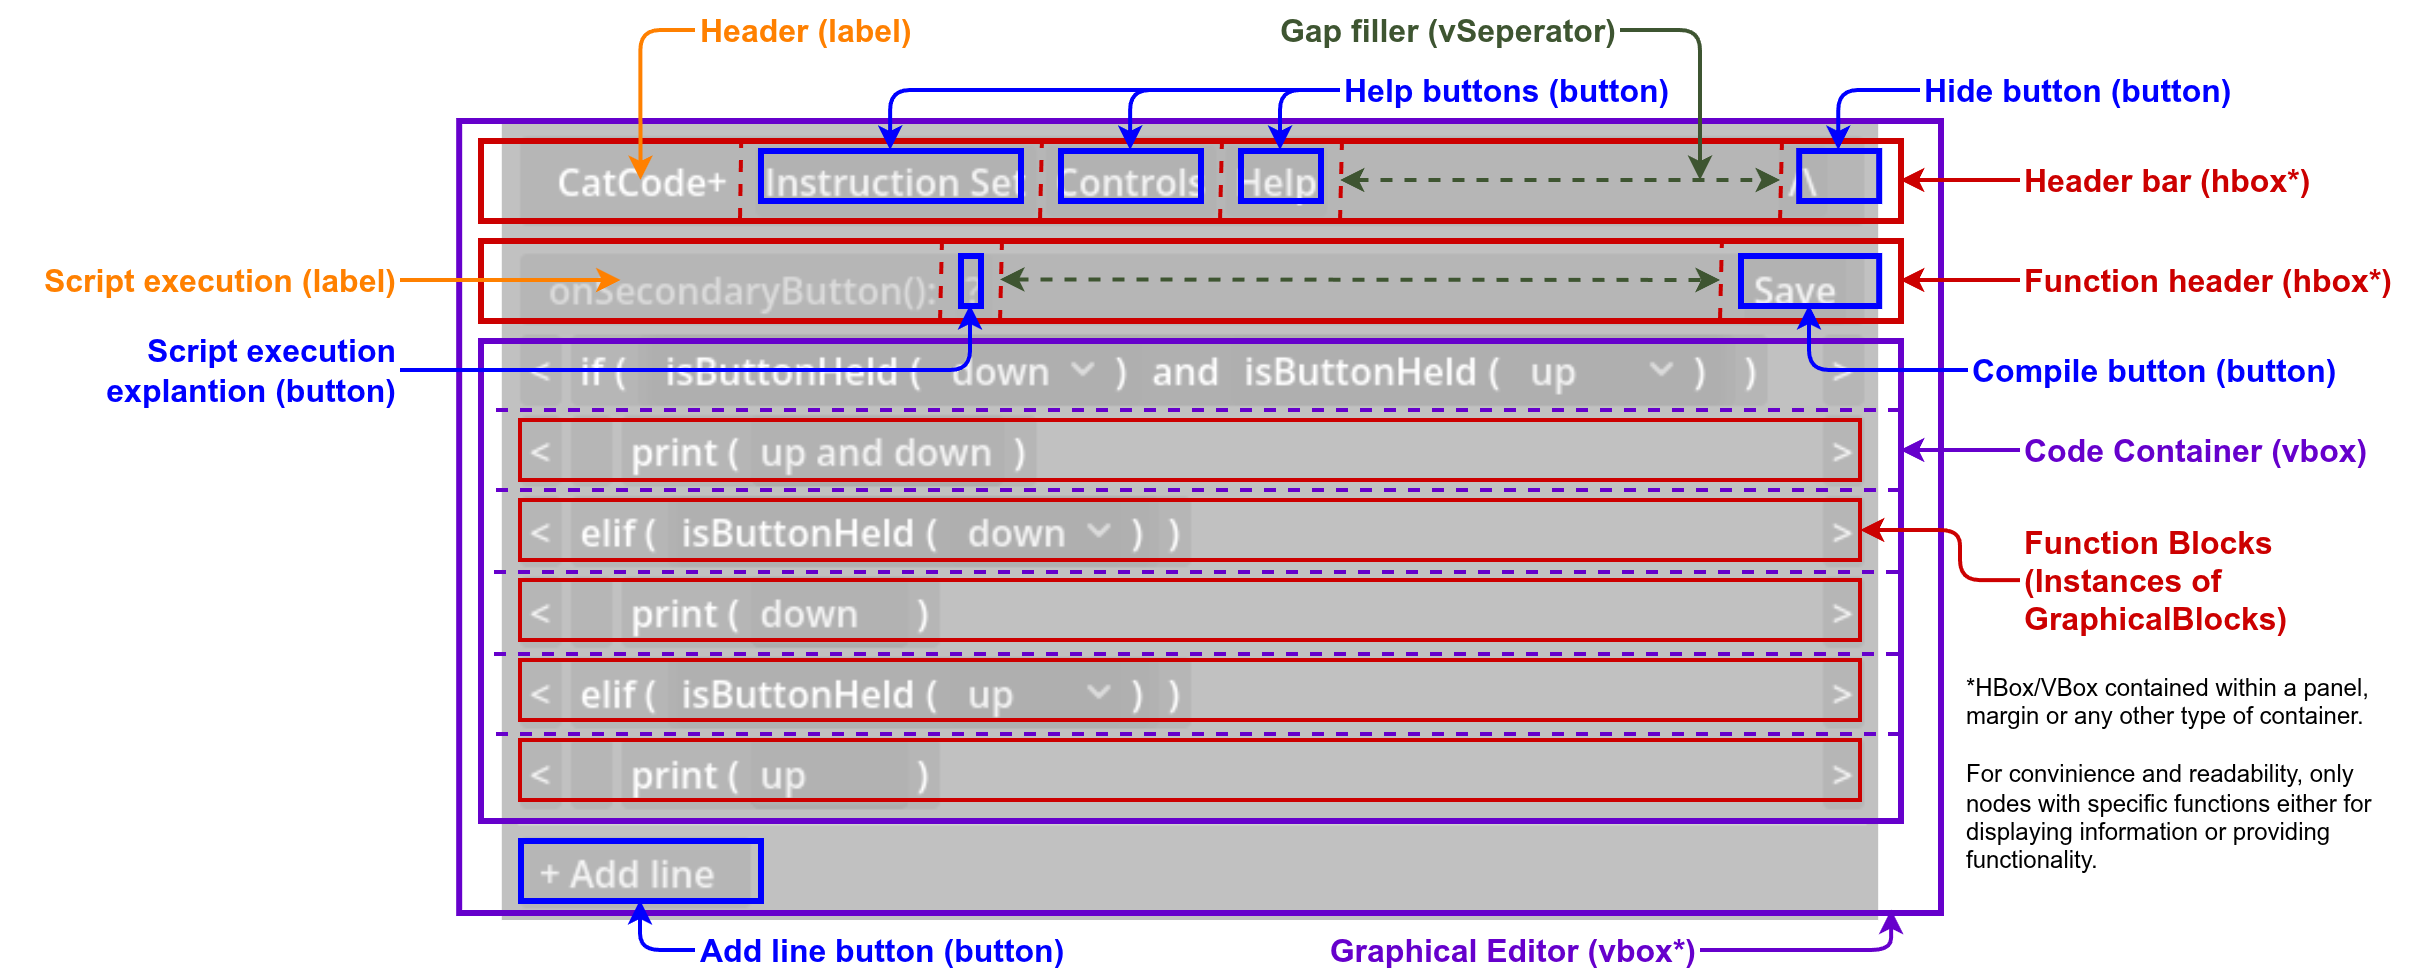
\includegraphics[width=1\linewidth]{C5/GraphicalCatCode/GraphicalEditorDiagram.drawio.png}
    \caption{Node structure of the basic graphical editor}
    \label{fig:design/catCode-graphicalEditor-Nodes}
\end{fullwidthfigure}

\begin{fullwidthfigure}
    \centering
    \begin{subfigure}[T]{1\linewidth}
        \centering
        \begin{tabular}{lll}\toprule
             Name & Contents & Composition \\\midrule
             Graphical Block* & Generic block with no parameters & [<id>] \\
             GB 1 FakeParam & Block with only a hidden parameter & [<id> <fk>] \\
             GB 1 OpenPositiveIntBox & Block with single positive number parameter & [<id> (<int>)] \\
             GB 1 Operand & Block with single operand, for blocks such as \texttt{if} & [<id> (<op>)] \\
             GB 1 StengthParam & Block with parameter between \texttt{0.0} and \texttt{1.0} & [<id> (<00\%>)] \\
             GB 1 TextBox & Block with a single textbox & [<id> (<txt>)] \\
             GB 2 TextBox & Block with two textboxes & [<id> (<txt>,<txt>)] \\ \midrule
             Basic Operand* & Generic operand with only a label & [<id>] \\
             OP 1 DropDown & Operator with a drop down of options & [<id> (<dd>)] \\
             OP 1 OperandContainer & Operator with an operand container, used by \texttt{not} & [<id> <op>] \\
             OP 2 OperandContainers & Operator with 2 operand containers, used by \texttt{and} & [<op> <id> <op>] \\
             OP 1 TextBox & Operand with a single text parameter & [<id> (<txt>)]
        \\ \bottomrule\end{tabular}
        \caption[Table of graphical blocks]{Table of graphical blocks. *Used as a superclass for other blocks.}
        \label{fig:design/catCode-graphicalBlocksAndComponents-A}
    \end{subfigure}
    \begin{subfigure}[T]{0.6\linewidth}
        \centering
        \begin{tabular}{lll}\toprule
            id & Name & Use \\\midrule
            \texttt{--} & Basic indent node & Visual representation of indents \\
            \texttt{<id>} & Block auto identifier & Text showing blocks name \\
            \texttt{<dd>} & Drop down param & Drop-down for pre-defined options \\
            \texttt{<fk>} & Fake param & Fake parameter created to fix a bug \\
            \texttt{<int>} & Integer param & Self explanatory \\
            \texttt{<op>} & Operator container & Slot for boolean operator \\
            \texttt{<00\%>} & Stength parameter & Strength percentage value \\
            \texttt{<txt>} & Text box param & Self explanatory
        \\ \bottomrule\end{tabular}
        \caption[Table of graphical components]{Table of graphical components, id for use only within this figure}
        \label{fig:design/catCode-graphicalBlocksAndComponents-B}
    \end{subfigure}
    \caption{Graphical components and graphical blocks.}
    \label{fig:design/catCode-graphicalBlocksAndComponents}
\end{fullwidthfigure}

\subsection{Function Blocks}

Function blocks handle a line of catCode in its entirety, including display, indent and parameters. Function blocks are a family of nodes shown in \autoref{fig:design/catCode-graphicalBlocksAndComponents-A} (contained within \texttt{catCode/graphicalBlocks}) that inherent the scene/node \textit{graphicalBlock}, which are made of defined components (\texttt{catCode/graphicalComponents}), listed in \autoref{fig:design/catCode-graphicalBlocksAndComponents-B}. The composition of these blocks are also shown in \autoref{fig:design/catCode-graphicalBlocksAndComponents}.

\subsection{Operand Blocks}

Operand blocks are handled as components of their parent graphical block, similar to parameters, using the \textit{operandContainer} node. This handles to menu to add the new block, storing the operand(s), and compiling them. Similar to the back-end, these work like parameters.

\subsection{Building and Compiling}

The graphical editor stores the code in a semi-compiled state (\texttt{draft\_code}) at all times as well as the most recent fully compiled code. \texttt{Draft\_code} will always contain up to date function blocks, and is updated whenever new blocks are added, but may not contain up to date parameters. It operates off two main methods: \texttt{push\_code()} and \texttt{pull\_code()}, pseudocode in \autoref{fig:design/catCode-GUI-push} and \autoref{fig:design/catCode-GUI-pull}. Each \textit{graphicalBlock} also has a push and pull function which will either construct its parameters or convert them into compiled code (recursively when operators are involved). Every action can be reduced to pushing and pulling as shown in \autoref{fig:design/catCode-GUI-methods}.

References to \textit{logicBlocks} are stored in two arrays (\texttt{operand\_list} and \texttt{function\_list}) rather than one, this is done to separate blocks that can only exist as parameters of other blocks from function blocks for use within menus. When the instruction set is updated within \textit{CodeManager} it emits the signal \texttt{instructions\_updated}, which carries the new instruction set. The editor receives this and uses this to construct its own arrays.

Compiled code is similarly passed back to to the \textit{CodeManager} through the use of signals, although it is expected that the \textit{CodeManager} calls the \texttt{compile()} function. The communication between nodes is shown in squence diagrams in \autoref{fig:design/catCode-GUI-comms-1}, \ref{fig:design/catCode-GUI-comms-2} and \ref{fig:design/catCode-GUI-comms-3}.

\begin{fullwidthfigure}
    \centering
    \begin{subfigure}[t]{0.45\linewidth}
        \smaller{
        \begin{tcolorbox}[boxrule=0.25mm]300
            \begin{verbatim}
FUNC compile():
    clear compiled_code
    pull_code()
    compiled_code ← draft_code()
    emit code_recompiled(compiled_code)
ENDFUNC





            \end{verbatim}
        \end{tcolorbox}
        }
        \subcaption{\texttt{compile()}}
    \end{subfigure}
    \begin{subfigure}[t]{0.45\linewidth}
        \smaller{
        \begin{tcolorbox}[boxrule=0.25mm]
            \begin{verbatim}
FUNC add_line(func_list_ind):
    previous_indent ← get_prev_ind()
    new_line ← instruction_line.new(
        prev_indent,
        function_list[func_list_ind],
        []
    )
    pull_code()
    draft_code.append(new_line)
    push_code()
ENDFUNC
            \end{verbatim}
        \end{tcolorbox}
        }
        \subcaption{\texttt{add\_line()}}
    \end{subfigure}
    \begin{subfigure}[t]{0.45\linewidth}
        \smaller{
        \begin{tcolorbox}[boxrule=0.25mm]
            \begin{verbatim}
FUNC set_code(new_code):
    draft_code ← new_code
    push_code
ENDFUNC

            \end{verbatim}
        \end{tcolorbox}
        }
        \subcaption{\texttt{set\_code()}}
    \end{subfigure}
\begin{subfigure}[t]{0.45\linewidth}
        \smaller{
        \begin{tcolorbox}[boxrule=0.25mm]
            \begin{verbatim}
FUNC remove_line(line):
    pull_code()
    draft_code.remove_at(line)
    push_code()
ENDFUNC
            \end{verbatim}
        \end{tcolorbox}
        }
        \subcaption{\texttt{remove\_line()}}
    \end{subfigure}    
    \caption{Graphical editor main functions (pseudocode)}
    \label{fig:design/catCode-GUI-methods}
\end{fullwidthfigure}

\begin{fullwidthfigure}
    \centering
    \begin{subfigure}[t]{1\linewidth}
        \begin{tcolorbox}[boxrule=0.25mm]
        \subcaption{\textbf{Graphical editor} (\texttt{res://src/catCode/ui/basic\_graphical\_editor.gd})}
        \smaller{
        \begin{verbatim}
func push_code():
    clear_nodes()
    print("> Pushing code...")
    for i in range(0, len(draft_code)):
        print("- " + str(i) + " " + str(draft_code[i]))
        var this_logic_block :logic_block = draft_code[i].primary_block
        var this_graphical_block :graphical_block = this_logic_block.ui_block.instantiate()
        this_graphical_block.code_editor = self
        instruction_nodes.append(this_graphical_block)
        code_container.add_child(this_graphical_block)
        this_graphical_block.bind_from_instruction(draft_code[i], i)
        \end{verbatim}
        }
        \end{tcolorbox}
    \end{subfigure}
    \begin{subfigure}[t]{1\linewidth}
        \begin{tcolorbox}[boxrule=0.25mm]
        \subcaption{\textbf{Graphical block} (\texttt{res://src/catCode/graphicalBlocks/graphical\_block.gd})}
        \smaller{
        \begin{verbatim}
func bind_from_instruction(instruction :instruction_line, _line_number :int = 0):
    consituent_block = instruction.primary_block
    indentifier = consituent_block.block_ref
    params = instruction.parameters
    indent = instruction.indent
    line_number = _line_number
    refresh_content()
        \end{verbatim}
        }
        \textbf{\textit{\#} \texttt{refresh\_content()} \textit{in turn calls} \texttt{push\_params()}\textit{, alongside emitting the relevant signals for the UI.}}

        \vspace{0.6cm}

        \begin{verbatim}
func push_params(will_emit_signal :bool = false):
    for i in range(0, len(params)):
        print("      " + str(parameter_nodes[i]))
        parameter_nodes[i].set_param_value(params[i])
    
    refresh.emit()
    if will_emit_signal: parameters_updated.emit(line_number, params)
        \end{verbatim}
        
        \end{tcolorbox}
    \end{subfigure}
    \caption{Push code functions}
    \label{fig:design/catCode-GUI-push}
\end{fullwidthfigure}

\begin{fullwidthfigure}
    \centering
    \begin{subfigure}[t]{1\linewidth}
        \begin{tcolorbox}[boxrule=0.25mm]
        \subcaption{\textbf{Graphical editor} (\texttt{res://src/catCode/ui/basic\_graphical\_editor.gd})}
        \smaller{
        \begin{verbatim}
func pull_code():
    clear_draft_code()
    print("> Pulling code...")
    for i in range(0, len(instruction_nodes)):
        print("- " + str(i) + " " + str(instruction_nodes[i]))
        draft_code.append(instruction_nodes[i].get_instruction_line())
        \end{verbatim}
        }
        \end{tcolorbox}
    \end{subfigure}
    \begin{subfigure}[t]{1\linewidth}
        \begin{tcolorbox}[boxrule=0.25mm]
        \subcaption{\textbf{Graphical block} (\texttt{res://src/catCode/graphicalBlocks/graphical\_block.gd})}
        \smaller{
        \begin{verbatim}
func get_instruction_line():
    return instruction_line.new(indent, consituent_block, get_params())

func get_params():
    pull_params(false)
    return params

func pull_params(will_emit_signal :bool = false) -> Array:
    params = []
    for this_parameter_node in parameter_nodes:
        params.append(this_parameter_node.get_param_value())
    
    if will_emit_signal: parameters_updated.emit(line_number, params)
    return params
        \end{verbatim}
        }
        \textbf{\textit{Each GraphicalComponent has a method} \texttt{get\_param\_value()} \textit{which returns a formatted list of parameters}}
        \end{tcolorbox}
    \end{subfigure}
    \caption{Pull code functions}
    \label{fig:design/catCode-GUI-pull}
\end{fullwidthfigure}

\begin{figure}
    \centering
    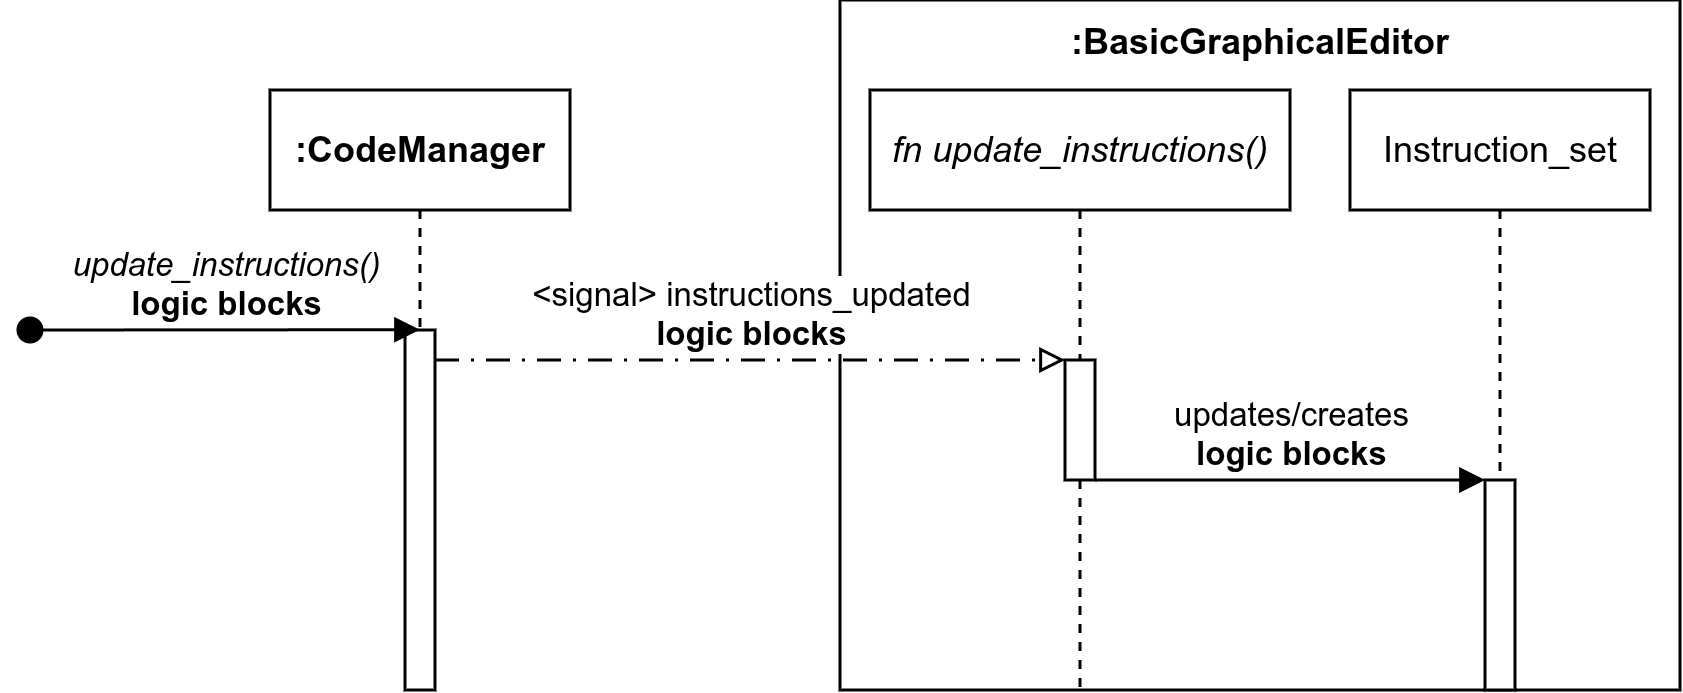
\includegraphics[width=0.75\linewidth]{C5//GraphicalCatCode/CatCodeGUI-communication-New-instructions.drawio.png}
    \caption{Sequence diagram of updating an instruction set}
    \label{fig:design/catCode-GUI-comms-1}
\end{figure}

\begin{figure}
    \centering
    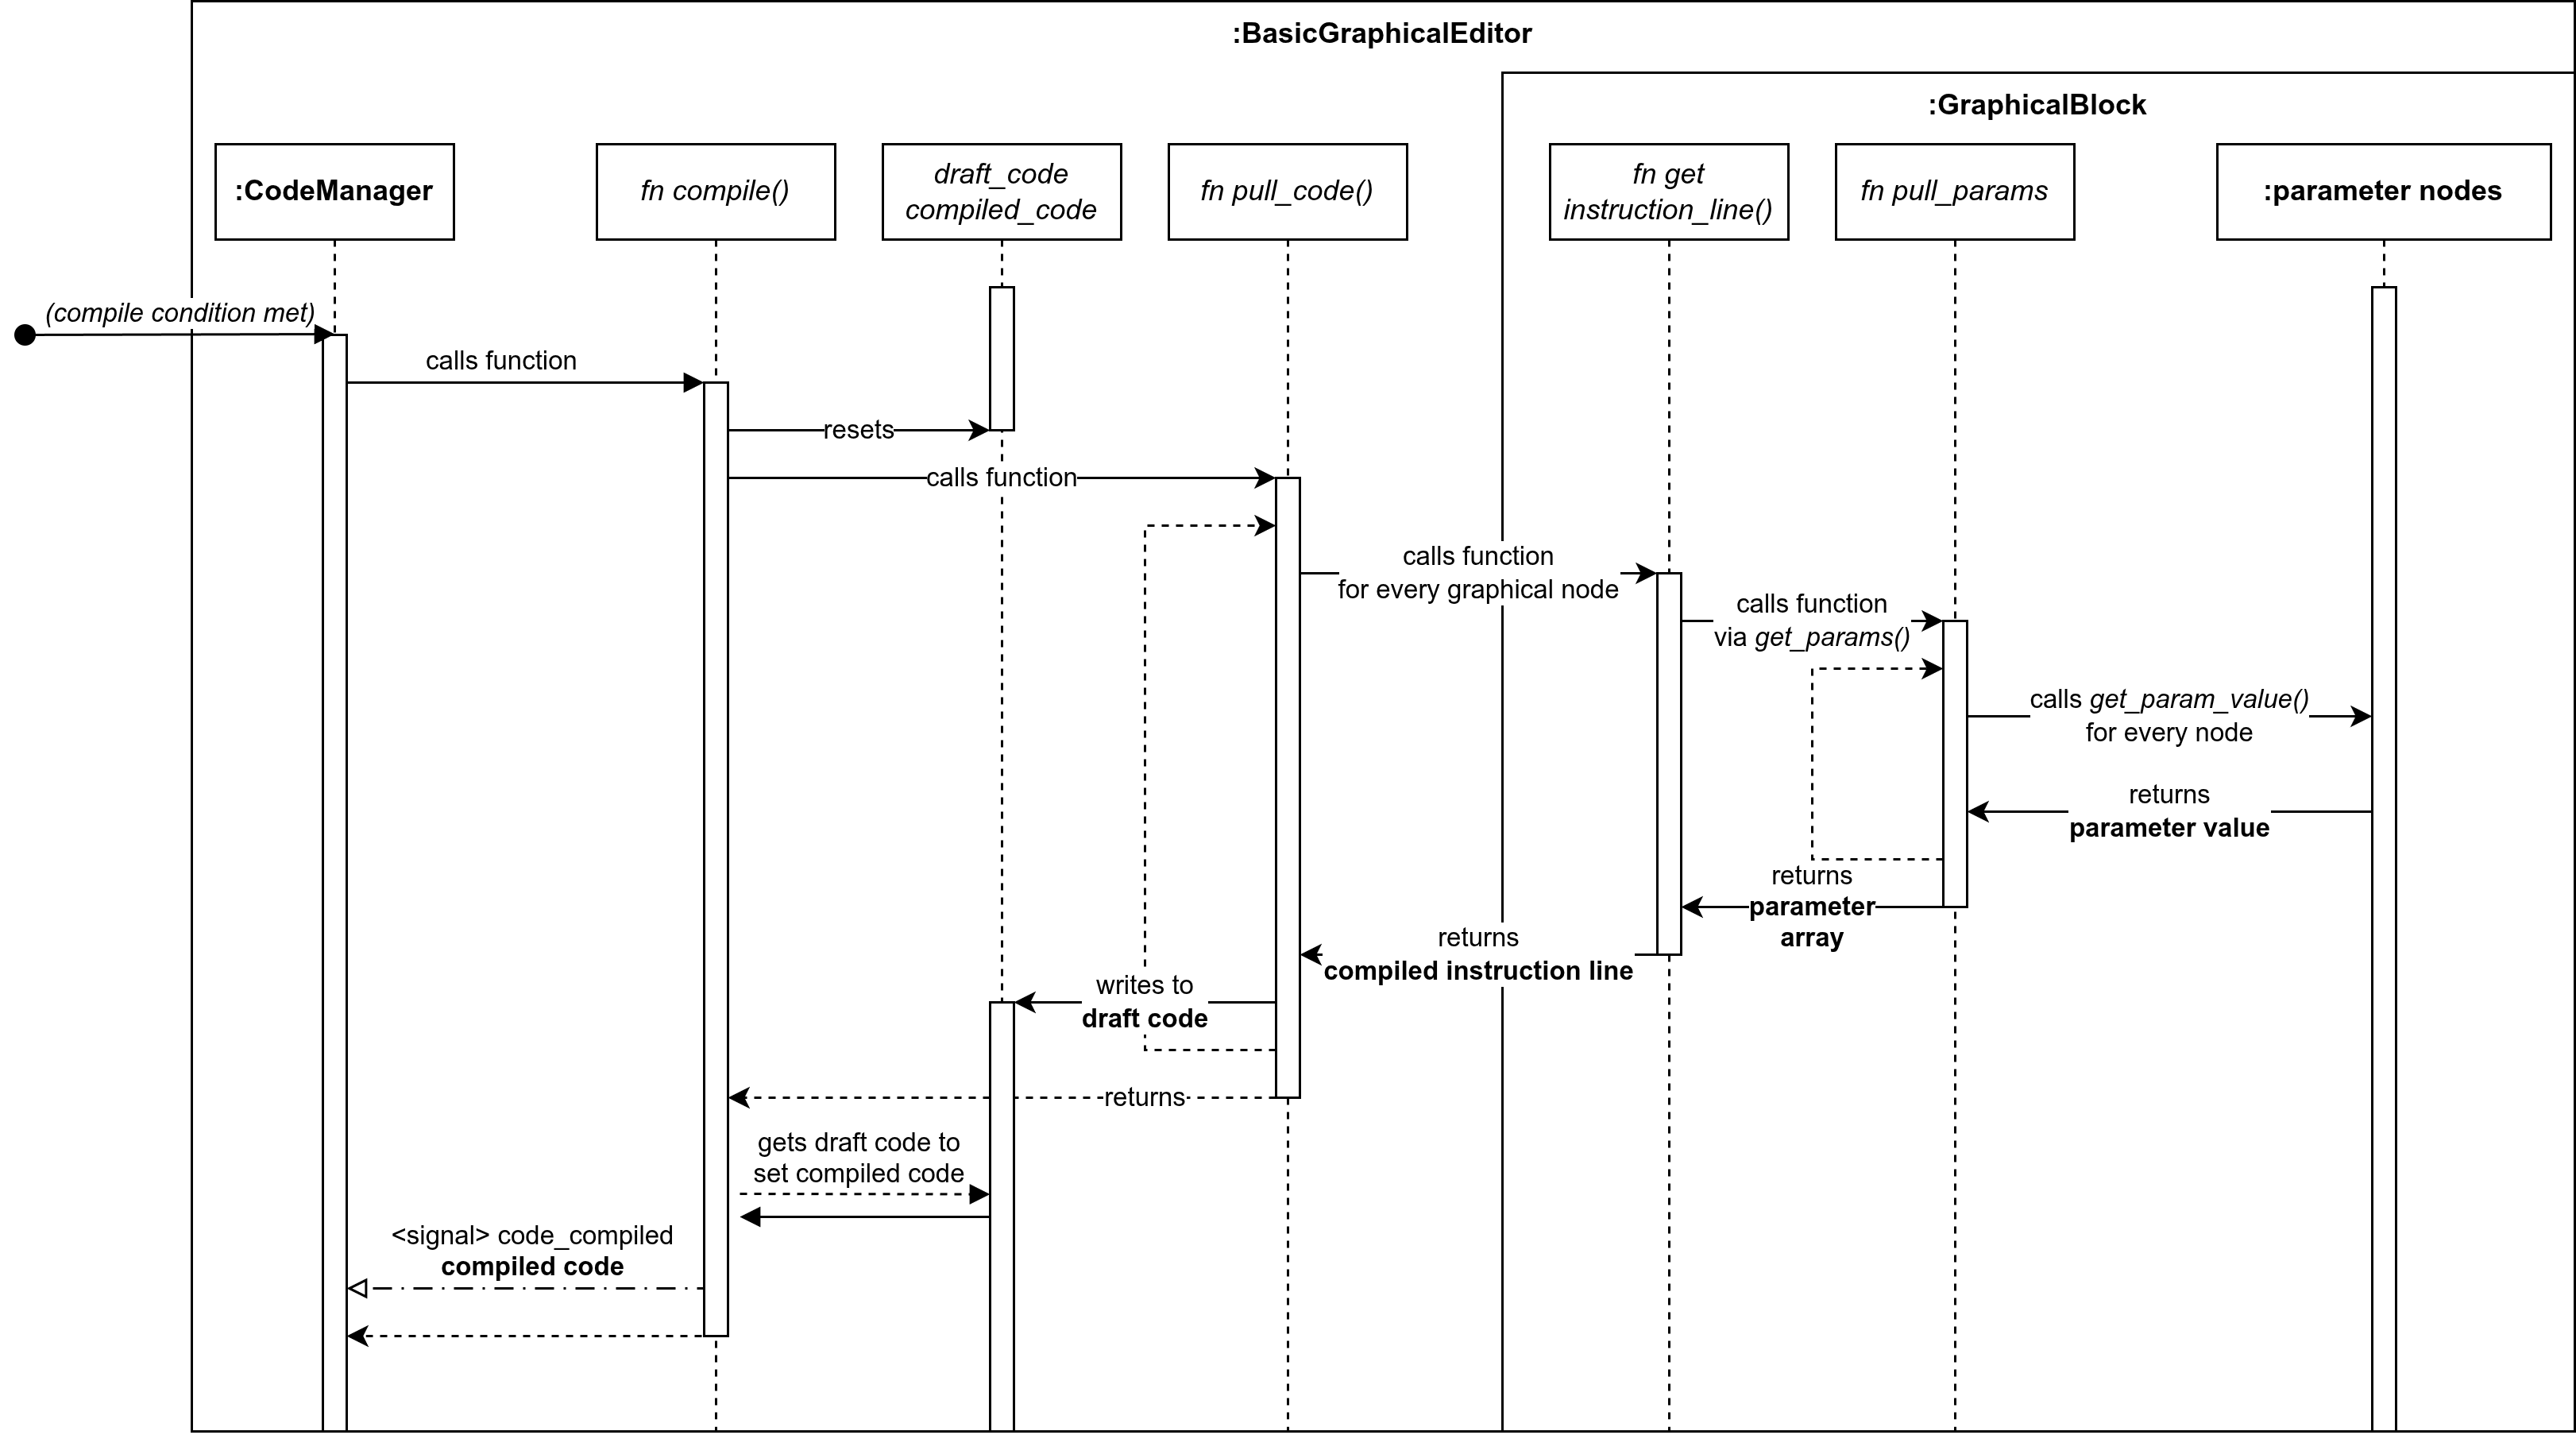
\includegraphics[width=1\linewidth]{C5//GraphicalCatCode/CatCodeGUI-communication-compileCode.drawio.png}
    \caption{Sequence diagram of compiling graphical CatCode}
    \label{fig:design/catCode-GUI-comms-2}
\end{figure}

\begin{figure}
    \centering
    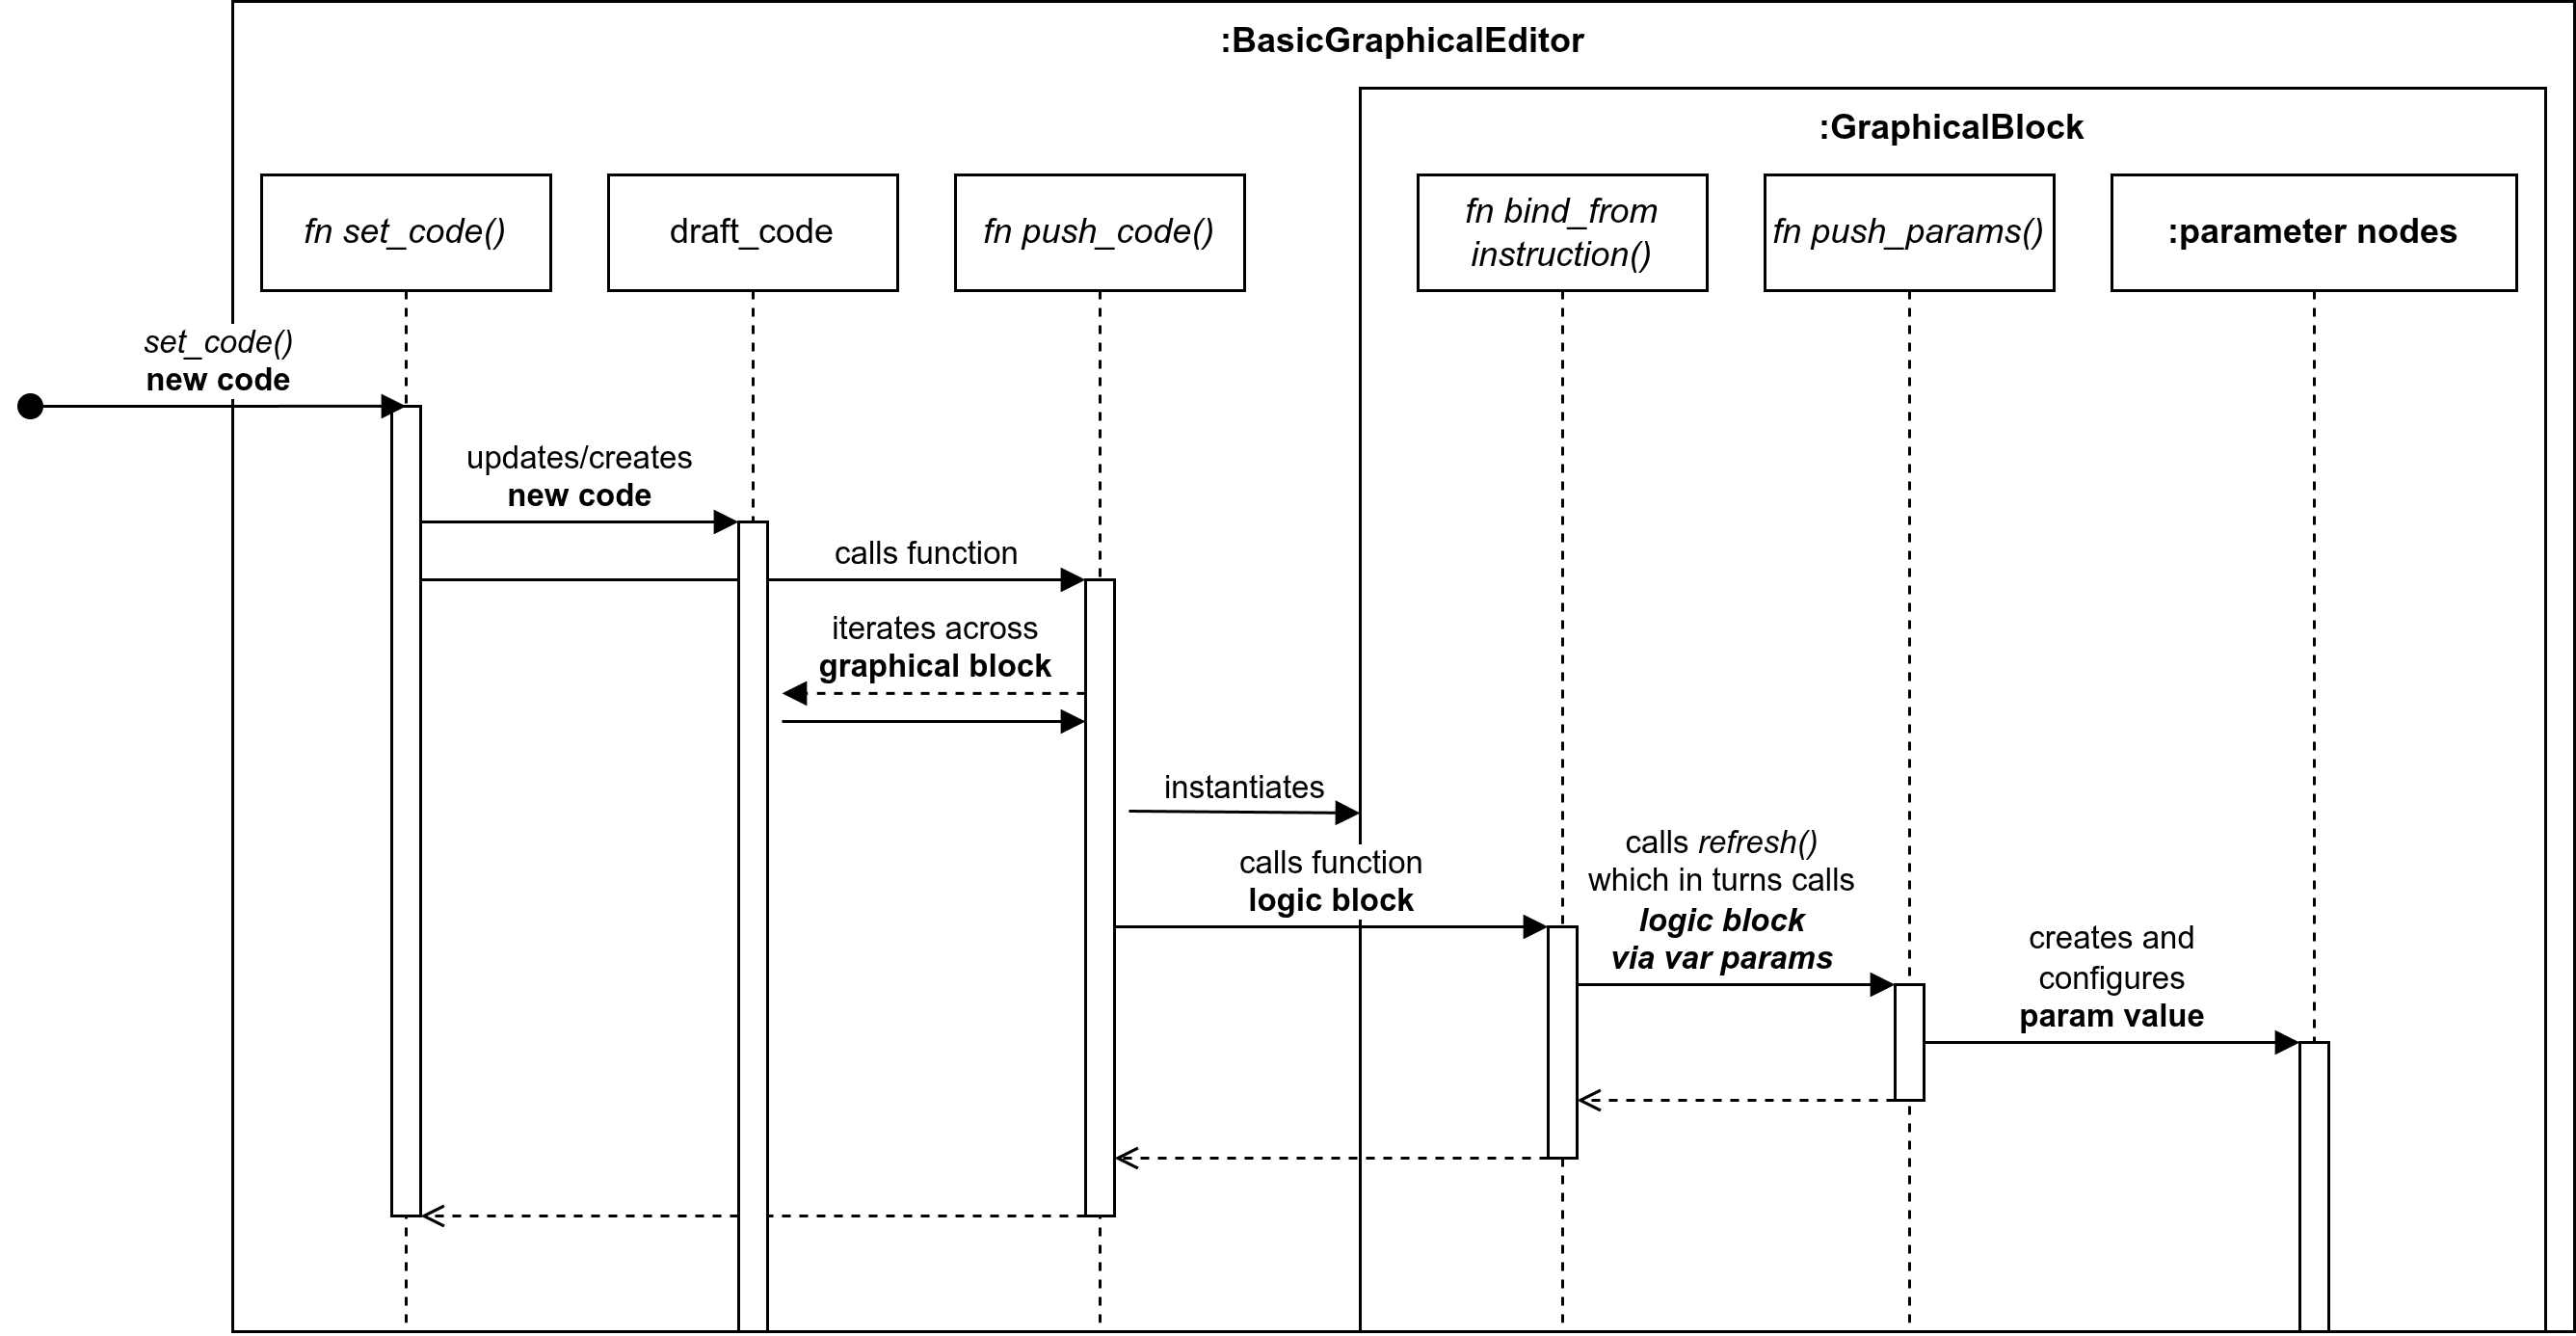
\includegraphics[width=1\linewidth]{C5//GraphicalCatCode/CatCodeGUI-communication-set-code.drawio.png}
    \caption{Sequence diagram of setting compiled CatCode to a new value}
    \label{fig:design/catCode-GUI-comms-3}
\end{figure}